\section{Preliminary Evaluation}

We built a FUSE-based middleware filesystem prototype and tested its metadata
performance on a
64-node cluster of dual core machines with 16GB memory interconnected with one 
GigE NIC.
Each node had a \giga{} indexing server process that managed its own \ldb instance 
that was stored on a local disk running Linux Ext3 file system.
This hardware does not have HPC-class networking or cluster file system, so our
preliminary experiments exclusively used metadata-intensive microbenchmarks.
To emulate shared storage for split operations, we used a NFS-mounted
volume accessible from all machines; this volume was only used for 
our cross-server \ldb split optimization.
We evaluated the performance of a single-node \ldb-based metadata store and
the scalability of our distributed middleware on 64 nodes.

We first evaluated the performance of a single-node \ldb-based metadata store
by running a test that creates 100 million zero-length files in a single
directory.
%To see the scalability of \ldb-based metadata store for supporting large directories,
%we run a test that creates 100 million zero-length files in a single directory,
Figure \ref{graph:ldb-singlenode} compares the instantaneous throughput of \ldb-based metadata 
store with three Linux file systems: Ext4 \cite{Ext4}, XFS \cite{XFS}, and
BTRFS \cite{BTRFS}.
%Figure \ref{graph:ldb-singlenode} shows a throughput timeline during the test. 
All systems perform well at the beginning of the test, but the file create
throughput drops gradually for all systems. 
BTRFS suffers the most serious throughput drop, slowing down to 100 operations 
per second. 
The \ldb-based store, however, maintains a more steady performance 
with an average speed of 2,200 operations per second respectively,
\textit{and is 10X faster than all other tested file systems.}

\begin{figure}[t]  %%%%%%%%%%%%%%%%%%%%%%%
\centerline{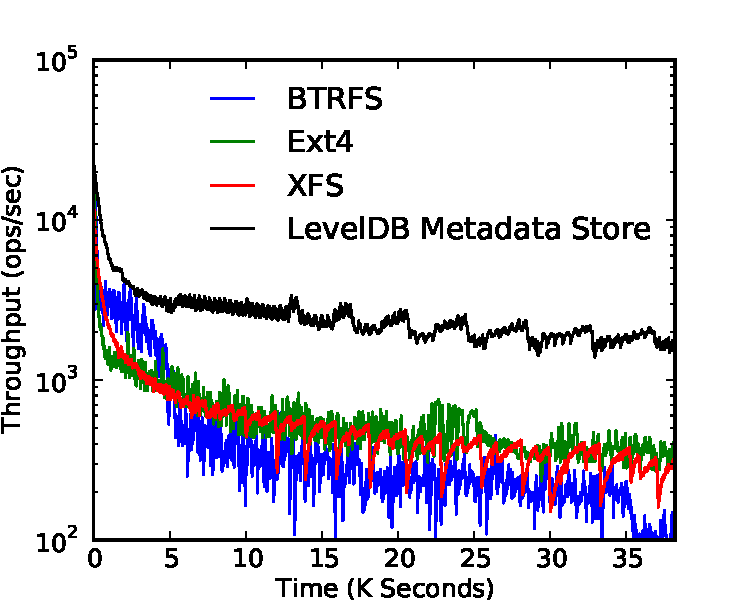
\includegraphics[scale=0.5]{./figs/ldb_insertrate_onenode}}
\caption{\normalsize
Single-node \ldb{}-based metadata store is 10X faster than modern Linux
filesystems for a workload that creates 100 million zero-length files.
X-axis only shows the time until LevelDB finished all insertions because the other 
file systems were much slower. Y-axis has a logarithmic scale.
}
\vspace{10pt}
\hrule 
\label{graph:ldb-singlenode}
\end{figure}       %%%%%%%%%%%%%%%%%%%%%%%


Next, we evaluated the scalability of our distributed metadata middleware
prototype.
Figure \ref{graph:ldb-scaling} shows the instantaneous throughput during the 
\textit{concurrent create} workload in a strong scaling experiment, i.e.
creating 1 million files per server, for a total of 64 million files in the
64-server configuration.
The main result in this figure is that as the number of servers doubles the
throughput of the system also scales up. With 64 servers, \giga{} can achieve a
peak throughput of about 190,000 file creates per second. The prototype delivers
peak performance after the directory workload has been spread among all
servers.
Reaching steady-state, the throughput quickly grows due to the splitting
policies adopted by \giga{}.

After reaching the steady state, throughput slowly drops as \ldb builds a
larger metadata store.
%Another observation in Figure \ref{graph:ldb-scaling} is that the system is
%unable to sustain the steady-state peak throughput (similar to our observation
%in the single-node test in Figure \ref{graph:ldb-singlenode}): 
In fact, in large setups with 8 or more servers, 
the peak throughput drops by as much as 25\% (in case of the 64-server setup).
This is because when there are more entries already existing in \ldb, 
it requires more compaction work to maintain \ldb invariants and to perform a 
negative lookup before each create has to search more SSTables on disk. 
In theory, the work of inserting a new entry to a LSM-tree is $O(\log_{B}(n))$
where $n$ is the total number of inserted entries, and $B$ is a constant factor
proportional to the average number of entries transferred in each disk request
\cite{Bender2007}.
Thus we can use the formula $\frac{a\cdot S+b}{\log{T}}$ to
approximate the throughput timeline in Figure \ref{graph:ldb-scaling},
where $S$ is the number of servers, $T$ is the running time, and $a$ as well as $b$ 
are constant factors relative to the disk speed and splitting overhead.
This estimation projects that when inserting 64 billion files with 64 servers,
the system may deliver an average of 1,000 operations per second per server,
i.e. 64,000 operations per second in aggregate.

\begin{figure}[t]  %%%%%%%%%%%%%%%%%%%%%%%
\centerline{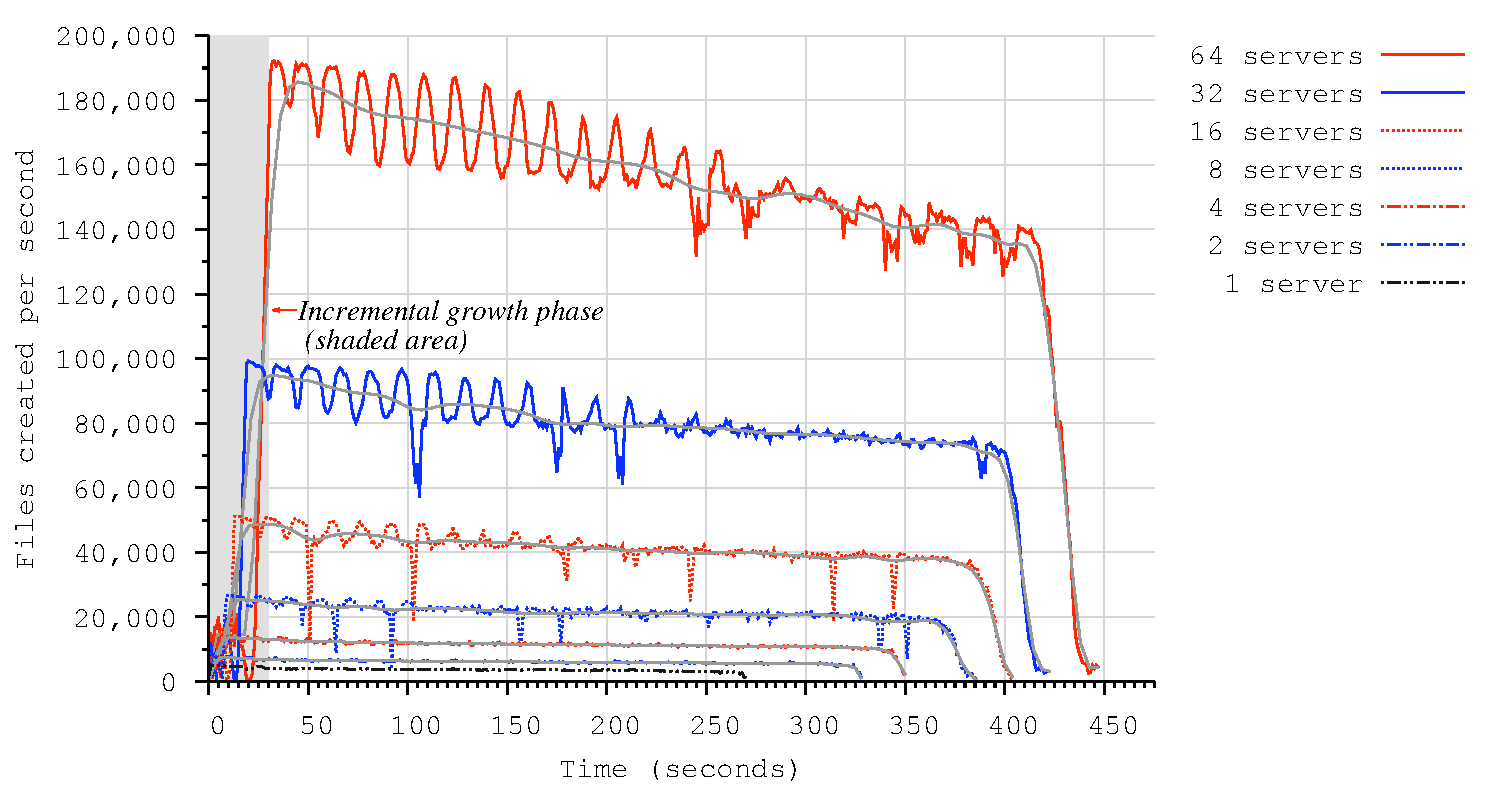
\includegraphics[scale=0.33]{./figs/ldb_insertrate}}
\caption{\normalsize
Our middleware metadata service prototype shows promising scalability
up to 64 servers. 
%However the interaction between LevelDB's compaction policies and 
%the Linux Ext3's implementation policies causes periodic throughput variance
%that degrades as the the number of directory entries in each LevelDB
%increases. 
Note that the solid lines in each configuration are Bezier
curves to smooth the variability.
}
\vspace{10pt}
\hrule 
\label{graph:ldb-scaling}
\end{figure}       %%%%%%%%%%%%%%%%%%%%%%%

